\documentclass{beamer}
\usepackage{moreverb} 
\usepackage{listings}
\usepackage{mflogo}
% imprimir
% \documentclass[handout]{beamer} 
% \usepackage{pgfpages}
% \pgfpagesuselayout{4 on 1}[a4paper,landscape,border shrink=5mm]

\mode<presentation> {
  \usetheme{Warsaw}
  \setbeamercovered{transparent}
}

\usebackgroundtemplate{
\includegraphics[width=\paperwidth]{format/libresoft-bg.png}}
% \usepackage[spanish]{babel}
\usepackage[utf8]{inputenc}
\usepackage{graphics}
\usepackage{amssymb} % Simbolos matematicos

%%%%%%%%%%%%%%%%%%%%%%%%%%%%%%%%%%%%%%%%%%%%%%%%%%%%%%%%%%%%%%%%%%%%%%%%%%%%%%%%%%%%%%%
%%
%% alert for highlighting
%% textit for Italic
%% texttt for URLs, etc
%%
%%%%%%%%%%%%%%%%%%%%%%%%%%%%%%%%%%%%%%%%%%%%%%%%%%%%%%%%%%%%%%%%%%%%%%%%%%%%%%%%%%%%%%%

%% Metadatos del PDF.
\hypersetup{  
  pdftitle={Vim editor},
  pdfauthor={Pedro Coca},
  pdfcreator={GSyC/Libresoft},
  pdfproducer=PDFLaTeX,
  pdfsubject={Master on Free Software},
}
%%

\defbeamertemplate*{footline}{shadow theme}
{%
  \leavevmode%
  \hbox{\begin{beamercolorbox}[wd=.5\paperwidth,ht=2.5ex,dp=1.125ex,leftskip=.3cm plus1fil,rightskip=.3cm]{author in head/foot}%
    \usebeamerfont{author in head/foot}\insertframenumber\,/\,\inserttotalframenumber\hfill
\includegraphics[scale=0.40]{format/cc-by-80x15.png} \hspace{0.1cm}\insertshortauthor 
% \usebeamerfont{author in head/foot} 
\includegraphics[width=0.7cm]{format/cc-by.png} \hfill\insertshortauthor
  \end{beamercolorbox}%
  \begin{beamercolorbox}[wd=.5\paperwidth,ht=2.5ex,dp=1.125ex,leftskip=.3cm,rightskip=.3cm plus1fil]{title in head/foot}%
    \usebeamerfont{title in head/foot}\insertshorttitle%
  \end{beamercolorbox}}%
  \vskip0pt%
}

\begin{document}

\title{Vim in a Nutshell}
\subtitle{Master on Libre Software 2011-12}
\institute{\texttt{http://master.libresoft.es} \\ Identi.ca - Twitter: \texttt{@mswl}}
\author{Pedro Coca} 
%\date{\today}
\date{October 20th, 2011}

\frame{
\maketitle
\begin{center}

\includegraphics[width=6cm]{format/gsyc-urjc}
\end{center}
}

%% License slide
\begin{frame}
  \vspace{2cm}
  \begin{center}
    {\small (cc) 2011 Pedro Coca, LibreSoft} \\
%    \vspace{0.25cm}
    \medskip
    {\scriptsize This work is licensed under \\ a Creative Commons Attribution 3.0 License}
%    \vspace{0.10cm}
  \end{center}
  \begin{center}
    \href{http://creativecommons.org/licenses/by/3.0/es}{
\includegraphics[width=2cm]{format/cc-by.png}} \\
    {\tiny \url{http://creativecommons.org/licenses/by/3.0}}
  \end{center}
\end{frame}%%

\usebackgroundtemplate{}

\AtBeginSubsection[]
{
  \begin{frame}<beamer>{Table of Contents}
    \tableofcontents[currentsection,currentsubsection]
  \end{frame}
}

%%%%%%%%%%%%%%%%%%%%%%%%%%%%%%%%%%%%%%%%%%%%%%%%%%%%%%%%%%%%%%%%%%%%%%%
\section{Introduction}
%%%%%%%%%%%%%%%%%%%%%%%%%%%%%%%%%%%%%%%%%%%%%%%%%%%%%%%%%%%%%%%%%%%%%%%

\subsection{History}
\begin{frame}
\frametitle{History}

\begin{itemize}
\item Written by Bill Joy in 1976 at the University of California, Berkeley
\item Written as the visual mode for the ex
\item Bill Joy's ex 1.1 line editor was part of the first BSD Unix release (March 1978)
\item The name vi is derived from \textit{visual in ex}
\item 1979. Mark Horton added support for function keys, macros...
\item 1983. Vi was added to Bell Labs System V
\end{itemize}
\end{frame}

\begin{frame}
\frametitle{History (2)}
\begin{itemize}
\item 1988. Vim \textit{(Vi IMproved, originally Vi IMitation)} is written by Bram Moolenaar for the Amiga computer
\item 1991. Vim first public release: v1.14
\item Several releases in the last 20 years adding features, fixing bugs, etc.
\item Last stable release: 15th October 2010: Vim 7.3
\item Vim 7.3. Lua support, Python3 support, Blowfish encryption, persistent undo/redo
\end{itemize}

\end{frame}

%%%%%%%%%%%%%%%%%%%%%%%%%%%%%%%%%%%%%%%%%%%%%%%%%%%%%%%%%%%%%%%%%%%%%%%

\subsection{Why vi?}
\begin{frame}
\frametitle{Why vi?}

\begin{itemize}
\item The Single UNIX Specification specifies vi, so every conforming system must include it
\item Runs on all systems that can implement the standard C library
\item 2009. A survey of Linux Journal readers found that vi was the most widely used text editor among respondents (36\%)
\item Small and fast
\item Editor War!
\end{itemize}

\end{frame}

%%%%%%%%%%%%%%%%%%%%%%%%%%%%%%%%%%%%%%%%%%%%%%%%%%%%%%%%%%%%%%%%%%%%%%%

\subsection{Editor War}
\begin{frame}
\frametitle{Editor War Humor}

\begin{figure}
  \centering
	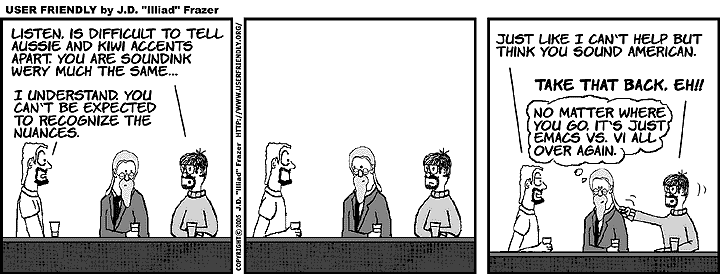
\includegraphics[scale=0.4,clip=true]{samples/editor_war.png}
  \label{fig:editor_war}
\end{figure}

\end{frame}


%%%%%%%%%%%%%%%%%%%%%%%%%%%%%%%%%%%%%%%%%%%%%%%%%%%%%%%%%%%%%%%%%%%%%%


\begin{frame}
\frametitle{Editor War Humor II}

\begin{figure}
  \centering
	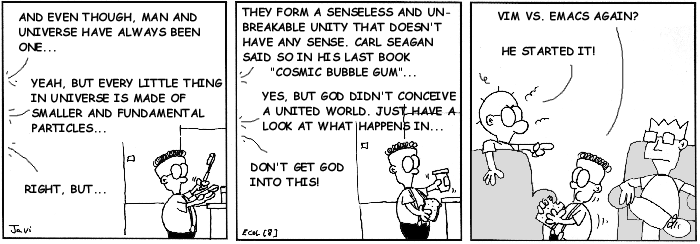
\includegraphics[scale=0.4,clip=true]{samples/editor_war_2.png}
  \label{fig:editor_war}
\end{figure}

\end{frame}



%%%%%%%%%%%%%%%%%%%%%%%%%%%%%%%%%%%%%%%%%%%%%%%%%%%%%%%%%%%%%%%%%%%%%%%

\subsection{Derivatives and clones}
\begin{frame}
\frametitle{Vi Derivatives and clones}

\begin{itemize}
\item \textbf{nvi}: version of vi that is shipped with all BSD-based open source distributions
\item \textbf{Vim}: Vi IMproved. More features than vim and included with most of the GNU/Linux distros.
\item \textbf{elvis}: Free vi clone for Unix and other OS
\item \textbf{vile}: Derived from Microemacs in an attempt to bring emacs editor paradigm to vi users
\item More comprehensive list at \textit{Vi Pages - Vi Clones and HomePages}
  \begin{itemize}
  \item \texttt{http://www.guckes.net/vi/clones.php3}
  \end{itemize}
\end{itemize}

\end{frame}

%%%%%%%%%%%%%%%%%%%%%%%%%%%%%%%%%%%%%%%%%%%%%%%%%%%%%%%%%%%%%%%%%%%%%%%

%%%%%%%%%%%%%%%%%%%%%%%%%%%%%%%%%%%%%%%%%%%%%%%%%%%%%%%%%%%%%%%%%%%%%%%

\section{Vi commands}

\subsection{Vi modes}

\begin{frame}
\frametitle{Vi modes}

\begin{itemize}
\item Vi is a modal editor
\item \textbf{Normal}: Command mode (AKA beep mode). Keystrokes are control commands
\item \textbf{Insert}: Insert / Replace text. Typed text is part of the document
\item \textbf{Visual}: In order to select a text piece
\item Escape key to return to Normal (command) mode
\end{itemize}

\end{frame}


%%%%%%%%%%%%%%%%%%%%%%%%%%%%%%%%%%%%%%%%%%%%%%%%%%%%%%%%%%%%%%%%%%%%%%%

\subsection{Moving around}

\begin{frame}
\frametitle{Navigating}
\begin{itemize}
\item \texttt{h j k l} move around the file
\item Arrow keys also move around the file
\item \texttt{w,W} go forward by word
\item \texttt{b,B} go backward by word
\item \texttt{e,E} go to then end of the word
\item \texttt{\$} and \texttt{0} go to the beginning and the end of a line
\item \texttt{\^} go to the first non blank character of the current line
\item \texttt{:<line\_number>} go to that line
\end{itemize}

\end{frame}

%%%%%%%%%%%%%%%%%%%%%%%%%%%%%%%%%%%%%%%%%%%%%%%%%%%%%%%%%%%%%%%%%%%%%%%

\subsection{Editing}

\begin{frame}
\frametitle{Inserting}
\begin{itemize}
\item \texttt{i} Insert text before cursor
\item \texttt{I} Insert text before the beginning of the line
\item \texttt{a} Insert text after cursor
\item \texttt{A} Insert text after the end of line
\item \texttt{o} Insert a new line for text below cursor
\item \texttt{O} Insert a new line for text above cursor
\end{itemize}

\end{frame}

%%%%%%%%%%%%%%%%%%%%%%%%%%%%%%%%%%%%%%%%%%%%%%%%%%%%%%%%%%%%%%%%%%%%%%%

\begin{frame}
\frametitle{Changing}
\begin{itemize}

\item \texttt{c motion} change text between the cursor and the target
\begin{itemize}
\item \texttt{cw} change word
\item \texttt{cc} change current line 
\item \texttt{c0} change text between the cursor and the beginning of line
\item \texttt{c\$} change text between the cursor and the end of line
\end{itemize}

\item \texttt{C} change text between the cursor and the end of line
\item \texttt{r} replace a single character
\item \texttt{R} Overwrite characters
\item \texttt{s} Substitute (delete the character and insert new text)
\item \texttt{S} Substitute line
\end{itemize}

\end{frame}

%%%%%%%%%%%%%%%%%%%%%%%%%%%%%%%%%%%%%%%%%%%%%%%%%%%%%%%%%%%%%%%%%%%%%%%

\begin{frame}
\frametitle{Deleting}
\begin{itemize}

\item \texttt{x} delete character under cursor
\item \texttt{X} delete character after cursor
\item \texttt{d motion} delete text between the cursor and the target
\begin{itemize}
\item \texttt{dw} delete word
\item \texttt{d5d} delete five (or n) lines
\item \texttt{dd} delete current line 
\item \texttt{d3d} delete three (or n) lines
\item \texttt{d0} delete text between the cursor and the beginning of line
\item \texttt{d\$} change text between the cursor and the end of line
\end{itemize}
\item \texttt{D} delete to the end of line
\item \texttt{p} put deleted text after the cursor
\item \texttt{P} put deleted text before the cursor
\end{itemize}

\end{frame}

%%%%%%%%%%%%%%%%%%%%%%%%%%%%%%%%%%%%%%%%%%%%%%%%%%%%%%%%%%%%%%%%%%%%%%%


\begin{frame}
\frametitle{Undoing and Redoing}

\begin{itemize}
\item \texttt{u} undo last action
\item \texttt{4u} undo last seven (or n) actions
\item \texttt{Ctrl+R} redo action
\item \texttt{4Ctrl+R} redo 4 (or n) actions
\end{itemize}

\end{frame}

%%%%%%%%%%%%%%%%%%%%%%%%%%%%%%%%%%%%%%%%%%%%%%%%%%%%%%%%%%%%%%%%%%%%%%%


\begin{frame}
\frametitle{Searching}

\begin{itemize}
\item \texttt{f<character>} search character in line
\item \texttt{F<character>} reverse search character in line
\item \texttt{/pattern} search forward pattern 
\item \texttt{?pattern} search backward pattern 
\item \texttt{n} repeat last search in same direction
\item \texttt{N} repeat last search in opposite direction
\item \texttt{:set hlsearch} /\texttt{nohlsearch} syntax highlighing (on/off)
\end{itemize}

\end{frame}

%%%%%%%%%%%%%%%%%%%%%%%%%%%%%%%%%%%%%%%%%%%%%%%%%%%%%%%%%%%%%%%%%%%%%%%

\begin{frame}
\frametitle{Substitute command}

\begin{itemize}
\item General syntax
\begin{itemize}
\item \textit{:[addr1[,addr2]]s/old/new/[flags]}
\item \textit{c flag} confirm each substitution
\item \textit{g flag} perform the substitution on each line (globally)
\end{itemize}
\item \textit{:s/old/new} replace next occurence of old with new in the current line
\item \textit{:s/old/new/g} replace all occurences of old with new in the current line
\item \textit{:\%s/old/new/g} replace all occurences of old with new in the current file
\item \textit{:30,130s/old/new/gc} replace all occurences of old with new in the lines 30 to 130 with confirmation

\end{itemize}

\end{frame}


%%%%%%%%%%%%%%%%%%%%%%%%%%%%%%%%%%%%%%%%%%%%%%%%%%%%%%%%%%%%%%%%%%%%%%%

\begin{frame}
\frametitle{Regular expressions}

\begin{itemize}
\item Vim uses mostly the same regular expresions than other unix programs, such as \textbf{grep}, \textbf{sed} and \textbf{awk}.
\item \texttt{.} single character
\item \texttt{*} matches zero or more characters
\item \texttt{\^} beginning of the line
\item \texttt{\$} end of the line
\item \texttt{\textbackslash} escapes the following character
\item \texttt{[ ]} matches any of the characters enclosed between brackets
\end{itemize}

\end{frame}


%%%%%%%%%%%%%%%%%%%%%%%%%%%%%%%%%%%%%%%%%%%%%%%%%%%%%%%%%%%%%%%%%%%%%%%


\begin{frame}
\frametitle{Regular expressions}

\begin{itemize}
\item Regular expresions are a complex topic
\item POSIX Bracket expressions
\begin{itemize}
\item \texttt{[:alnum:]} matches alphanumeric characters
\item \texttt{[:alpha:]} matches alphabetic characters
\item \texttt{[:blank:]} matches space and tab characters
\item \texttt{[:space:]} matches whitespace characters
\item ...
\end{itemize}
\end{itemize}

\end{frame}


%%%%%%%%%%%%%%%%%%%%%%%%%%%%%%%%%%%%%%%%%%%%%%%%%%%%%%%%%%%%%%%%%%%%%%%

\begin{frame}
\frametitle{Multiple Windows}

\begin{itemize}
\item \texttt{vim -o2 file1 file2} open both files in windows
\item \texttt{:split} split horizontally the window
\item \texttt{:split filename} split horizontally and display filename
\item \texttt{:vsplit} split vertically the window
\item \texttt{CRTL+W} Window Navigation
\begin{itemize}
\item \texttt{h,j,k,l} Moving around
\item \texttt{arrow keys} Moving around
\end{itemize}
\item Windows can also be resized and moved.
\end{itemize}

\end{frame}

%%%%%%%%%%%%%%%%%%%%%%%%%%%%%%%%%%%%%%%%%%%%%%%%%%%%%%%%%%%%%%%%%%%%%%%

\begin{frame}
\frametitle{Write and exit}

\begin{itemize}
\item \texttt{:w} write to file
\item \texttt{:q} quit (will notice us if there is no write since last change)
\item \texttt{:q!} quit without any notice
\item \texttt{:wq} write to file and quit 
\end{itemize}

\end{frame}

%%%%%%%%%%%%%%%%%%%%%%%%%%%%%%%%%%%%%%%%%%%%%%%%%%%%%%%%%%%%%%%%%%%%%%%

\begin{frame}
\frametitle{Cutting, Pasting, Copying}

\begin{itemize}
\item whenever you deleted or copy any piece of text is stored in a buffer
\item can be pasted with p or P
\item in visual mode we can select a piece of text and copy it with the yank command (y)
\item named buffers can be used: \textit{"x}
\begin{itemize}
\item \textit{"ayy} yanks the current line into buffer a 
\item \textit{"ap} puts the content of buffer a after cursor
\item If you use the capital letter for the buffer the content is appended to the current content
\end{itemize}
\end{itemize}

\end{frame}

%%%%%%%%%%%%%%%%%%%%%%%%%%%%%%%%%%%%%%%%%%%%%%%%%%%%%%%%%%%%%%%%%%%%%%%


\begin{frame}
\frametitle{Invoking the shell commands}

\begin{itemize}
\item \texttt{:!} executes a shell command
\item \texttt{:!!} execute again the last command
\item \texttt{:read filename} reads (and inserts) the content of the line after the cursor
\item \texttt{:\$r ! date} reads the date command of the shell and writes it at the end of current the file
\item \texttt{:90,99!sort} sort these lines!
\end{itemize}

\end{frame}



%%%%%%%%%%%%%%%%%%%%%%%%%%%%%%%%%%%%%%%%%%%%%%%%%%%%%%%%%%%%%%%%%%%%%%%


\begin{frame}
\frametitle{Miscelania}

\begin{itemize}
\item \texttt{J} join two lines
\item \texttt{5J} join five (or n) lines
\item \texttt{\~} change case
\item \texttt{5\~} change case for five (or n) characters
\item \texttt{.} Repeat last edit command
\item \texttt{:w !sudo tee \%} Read-only annoying issue
\end{itemize}

\end{frame}

%%%%%%%%%%%%%%%%%%%%%%%%%%%%%%%%%%%%%%%%%%%%%%%%%%%%%%%%%%%%%%%%%%%%%%%

\section{Configuration and customization}

\subsection{Files and commands}
\begin{frame}
\frametitle{Files and commands}

\begin{itemize}
\item We can enable and configure many features for our convenience
\item Line numbering, syntax color, Indentation, etc
\item Configuration files:
\begin{itemize}
\item For all Vim system users: \texttt{/etc/vim/vimrc}
\item For just our user: \texttt{\$HOME/.vimrc}
\end{itemize}
\item We can define options and parameters while editing:
\begin{itemize}
\item \texttt{:set <command>}
\end{itemize}

\end{itemize}

\end{frame}


%%%%%%%%%%%%%%%%%%%%%%%%%%%%%%%%%%%%%%%%%%%%%%%%%%%%%%%%%%%%%%%%%%%%%%%

\begin{frame}
\frametitle{Configuration commands}

\begin{itemize}
\item Some useful commands:
\begin{itemize}
\item \texttt{:set ic} / \texttt{:set noic} ignore case when searching (on/off)
\item \texttt{:set nu} / \texttt{:set nonu} display line numbers (on/off)
\item \texttt{:set ai} / \texttt{:set noai} set the auto indentation mode (on/off)
\end{itemize}
\item \texttt{:set all} command displays the list for all options
\end{itemize}

\end{frame}


%%%%%%%%%%%%%%%%%%%%%%%%%%%%%%%%%%%%%%%%%%%%%%%%%%%%%%%%%%%%%%%%%%%%%%%

\subsection{Plug-ins}
\begin{frame}
\frametitle{Plug-in}

\begin{itemize}
\item There are many plug-ins or extensions that will make some tasks easier.
\item NERD tree
  \begin{itemize}
  \item Flexible directory tree (Better than :Vex)
  \end{itemize}
\item VCS Command
  \begin{itemize}
  \item Manipulates files under CVS, SVN, GIT, etc.
  \item Changes and differences can be addressed (Vimdiff)
  \end{itemize}
\item snipMate 
  \begin{itemize}
  \item Snippets usage. Lets see an example
  \item \url{http://vimeo.com/3535418}
  \item and try it out!
  \end{itemize}
\end{itemize}

\end{frame}



%%%%%%%%%%%%%%%%%%%%%%%%%%%%%%%%%%%%%%%%%%%%%%%%%%%%%%%%%%%%%%%%%%%%%%%

\begin{frame}
\frametitle{Plug-in installation}

\begin{itemize}
\item Usually provided in .zip format
\item Unzip the plugin in the .vim directory (Linux)
\item Do not forget to enable them! 
\begin{itemize}
\item \textit{filetype plugin on}
\end{itemize}
\end{itemize}

\end{frame}





\begin{frame}
\frametitle{Conclusions}

\begin{itemize}
\item Vim is a very powerful and flexible editor
\item Vim's steep learning curve has to be taken into account
\item Vim requires a big investment in time
\item Editing skills save a lot of time
\item Many useful plugins than can save the day
\end{itemize}

\end{frame}


%%%%%%%%%%%%%%%%%%%%%%%%%%%%%%%%%%%%%%%%%%%%%%%%%%%%%%%%%%%%%%%%%%%%%%%
\section{References}
%%%%%%%%%%%%%%%%%%%%%%%%%%%%%%%%%%%%%%%%%%%%%%%%%%%%%%%%%%%%%%%%%%%%%%%

\begin{frame} 
\frametitle{References}

\begin{itemize}
\item Vim help! \textit{:help}
\item Vim documentation \url{http://www.vim.org/docs.php}
\item Wikibooks. Learning the vi editor \url{http://en.wikibooks.org/wiki/Learning\_the\_vi\_Editor}
\item Learning the vi and vim editors 7th Edition. (A. Robbins, E. Hannah and L. Lamb). O'Reilly. July 2008
\end{itemize}

\end{frame}

%%%%%%%%%%%%%%%%%%%%%%%%%%%%%%%%%%%%%%%%%%%%%%%%%%%%%%%%%%%%%%%%%%%%%%%

% Final slide
\usebackgroundtemplate{
\includegraphics[width=\paperwidth]{format/libresoft-bg}}

\frame{
\maketitle
\begin{center}

\includegraphics[width=6cm]{format/gsyc-urjc}
\end{center}
}

\end{document}

